
% JuliaCon proceedings template
\documentclass{juliacon}
\setcounter{page}{1}

\begin{document}

% **************GENERATED FILE, DO NOT EDIT**************

\title{My JuliaCon proceeding}

\author[1]{1st author}
\author[1, 2]{2nd author}
\author[2]{3rd author}
\affil[1]{University}
\affil[2]{National Lab}

\keywords{Julia, Optimization, Game theory, Compiler}

\hypersetup{
pdftitle = {My JuliaCon proceeding},
pdfsubject = {JuliaCon 2022 Proceedings},
pdfauthor = {1st author, 2nd author, 3rd author},
pdfkeywords = {Julia, Optimization, Game theory, Compiler},
}



\maketitle

\begin{abstract}

\verb|AdaptiveHierarchicalRegularBinning.jl| computes a hierarchical space-partitioning
tree for a given set of points of arbitrary dimensions, that divides the space and
stores the reordered points offering efficient access. Space-partitioning data
structures are vital for algorithms that exploit spatial distance to reduce
computational complexity, see for example the Fast Multipole Method, and algorithms
finding nearest neighbors and their applications.

\end{abstract}

\section{Overview}
To partition a cloud of points of $d$ dimensions,
\verb|AdaptiveHierarchicalRegularBinning.jl| maps each point to a $1$ dimensional
space filling curve, Morton or Z-order curve. The hierarchical tree is defined by the
Morton index of each point.



\subsection{Morton encoding}
Morton indices are binary words grouped into $l$ levels of $d$ bits each. Each level
describes in an increasingly finer detail the area in which the point resides. The
first level, comprised of the $d$ most significant bits of the morton index, describes
only in which half of each dimension the point lies.

$$b = \left\{\begin{matrix}
  (0)_2, & \textrm{Left-most half}  \\
  (1)_2, & \textrm{Right-most half}
\end{matrix}\right.$$


\begin{definition}[Left/Right-mostness]
  For a $1$-dimensional simply connected space $A = [m, M)$, we say that
  $x$ lies in the Left-most half, if and only if, $x<h=\frac{M+m}{2}$.
  Otherwise $x$ lies in the Right-most half.

  $$
  \begin{matrix}
    L &\triangleq& [m, h) \\
    R &\triangleq& [h, M)
  \end{matrix}
  $$
\end{definition}


\begin{example}[Morton index interpretation]
  Figure \ref{spatial-tree} depicts a $2$-dimensional space and a target spatial
  tree of at most $2$ levels (other than the root). The morton index, in such a tree,
  will have a length of $2\cdot2=4$. Assume we compute a morton index of $(0011)_2$.
  The first group is comprised of the $2$ most significant bits and addresses the first
  level of the tree (the one directly under root).
  \\\\
  The most significant bit addresses the first dimension and the second most significant
  bit addresses the second dimension. The value $(0)_2$ signifies that the point lies in
  the left-most half of each dimension.
  \\\\
  The next group describes the same quantities only a level lower. Left/Right-mostness
  is defined in the context of that level. Both values are $(1)_2$ so the point lies in
  the right-most half of both dimensions in the second level.
  \\\\
  Summarizing, the point belongs to the:
  \begin{itemize}
    \item right-most half of the left-most half of the first dimension.
    \item right-most half of the left-most half of the second dimension.
  \end{itemize}

  \begin{figure}
    \centerline{
      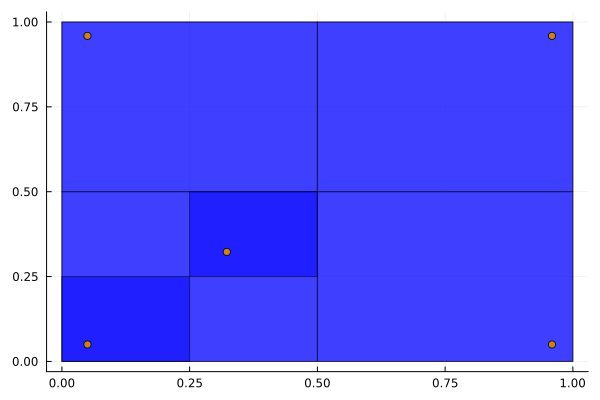
\includegraphics[width=10pc]{figures/spatial-division.png}
      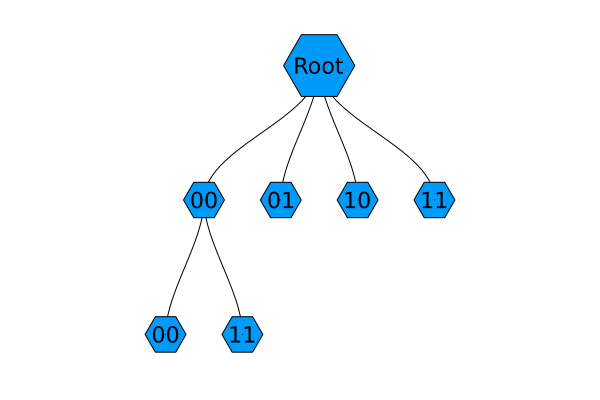
\includegraphics[width=10pc]{figures/spatial-tree.png}
    }
    \caption{ (a) Spatial division, (b) Spatial tree }
    \label{spatial-tree}
  \end{figure}
\end{example}

\subsection{Reordering}
Sorting in terms of the morton indices groups the points together for efficient access
when the tree is iterated over. We use the \verb|MSD Radixsort| algorithm to perform the
soring.

\subsubsection{MSD Radixsort}
\verb|MSD Radixsort| sorts based on the most significant radix. Afterwards, elements
with the same most significant digit (MSD) form a consecutive sub-array. The algorithm
recurses for each such sub-array selecting the next digit in line. Selecting a large
radix is crucial for the algorithm since a large radix lowers the number of recursions.
\\\\
\verb|MSD Radixsort| respects the hierarchical nature of the target tree and thus it offers
benefits over other sorting algorithms. Each recursion of the algorithm sorts a section
of the resulting tree. If the radix matches the number of dimensions then each recursion
sorts the current level of the tree.
\\\\
When the number of elements of a sub array is small the recursion for that sub-array stops.
This leads to a partialy sorted array by design. Not sorting small sub-arrays leads to less
overhead without sacrificing future performance. Nodes with unsorted morton indices will
always be leaf nodes.
\\\\
\verb|MSD Radixsort| can be trivialy parallelized. After the initial sorting, the formed
sub-arrays are mutually exclusive, meaning that no data dependencies are shared between
them. Each sub-array can then be sorted in parallel.

\subsubsection{Countsort}
\verb|MSD Radixsort| needs a sorting algorithm to sort the selected radix in each recursion.
\verb|Countsort| is a great fit for this type of sorting. \verb|Countsort| trades
space complexity for runtime complexity. The algorithm uses an auxilary vector, whose
size scales linearly with the selected radix $O(r)$. The benefit is the runtime
complexity is order $O(n + r)$ where $n$ is the size of the array to sort. Typically, $n \gg r$
and so the runtime complexity reduces to $O(n)$.
\\\\
\verb|Countsort| can be parallelized as well, though not as trivialy. The parallel version
of \verb|Countsort| requires space complexity of $O(t\cdot r)$ and runtime complexity of
$O(n/t + t\cdot r)$ where $t$ is the number of threads in the system. As long as $n$ is
sufficiently large $n \gg t^2\cdot r$ then the parallel implementation is preferable since
the runtime complexity reduces to $O(n/t)$.

\subsubsection{Radix trade-off}
While \verb|MSD Radixsort| fairs better for larger radices, \verb|Countsort| reduces in
performance.

\begin{example}
  For a $128$-bit morton index, a radix of $16$-bits is selected.
  The number of recursions in this case is $8$ which is fairly small and the condition
  $n\gg t^2\cdot r$ can still be satisfied.
  % TODO: Graphs runtime complexity vs r
\end{example}

Our implementation utilizes a watefall scheme to adapt to the needs of the problem at
hand. There are $3$ different thresholds that can tune the runtime performance of the
spatial partitioning.

\begin{itemize}
  \item \verb|Huge| threshold
  \item \verb|Big| threshold
  \item \verb|Small| threshold
\end{itemize}

$$ \textrm{Huge} > \textrm{Big} > \textrm{Small} $$

For sub-arrays that are larger than the \verb|Huge| threshold our implementation
uses parallel \verb|MSD Radixsort|, otherwise it falls back to the non parallel variant.
\\\\
For sub-arrays that are larger than the \verb|Big| threshold our implementation uses
parallel \verb|Countsort|, otherwise it falls back to the non parallel variant.
\\\\
For sub-arrays that are smaller than the \verb|Small| threshold our implementation
stops the recursion of \verb|MSD Radixsort|.


\subsection{Tree}
The resulting tree is memory-dense, meaning that it does not store empty nodes.
The root node encapsulates the entire cloud of points, while each child node points to
a consecutive sub-array of those points. This characteristic holds true for every node
within the tree. Each node is also aware if its level, parent and children.


\section{Usage}

\begin{lstlisting}[language = Bash]
  $ julia -t auto
\end{lstlisting}

\begin{lstlisting}[language = Julia]
  using AdaptiveHierarchicalRegularBinning
  n = 10000
  d = 5
  X = rand(n, d)

  tree = regular_bin(X, dpt, sml_th; dims=2)
  # X is no permuted to accomodate morton encoding

  for leaf in Leaves(tree)
  # iterates over the tree's leafs
  end

  for node in PreOrderDFS(tree)
    # iterates over the tree's nodes in pre order
  end

  I, D = knn(tree, X)

  original_perm!(tree, I, D)
  # I and D are now refering to the
  # original permutation
\end{lstlisting}


\section{Theory}
Assuming a set of $n$ $d$-dimensional points $\mathcal{V}$, we represent $\mathcal{V}$ as
the $d \times n$ matrix $V$. \verb|AdaptiveHierarchicalRegularBinning.jl| uses Morton
encoding to map each $d$-dimenensional point of $\mathcal{V}$ to a $1$-dimenensional
space filling curve, Z-order curve.
\\\\
The mapping proccess requires 3 distinct steps.

\begin{itemize}
  \item Normalize $\mathcal{V}$ such that each vector $\vec{v}$ of $\mathcal{V}$
  satisfies $\vec{v} \in [0,1)^d$.
  \item Quantize each dimension using an $l$-bit quantizer, where $l$ is the maximum
  depth of the target tree.
  \item Bit-interleave the output of the quantizer.
\end{itemize}

\subsection{Normalization}
In order to compute the hierarchical tree we first normalize $\mathcal{V}$.

$$ \vec{v} \in \mathcal{H}, \forall \vec{v} \in \mathcal{V}$$

Where $\mathcal{H}$ is the connected $d$-dimensional space that contains all vectors
of $\mathcal{V}$.

$$ H \triangleq [m_1, M_1] \times [m_2, M_2] \times \cdots \times [m_d, M_d] $$

Where
$$\space m_i = \min_j\left(V_{i,j}\right), \forall i \in \left\{1, 2, \cdots, d\right\}$$
$$\space M_i = \max_j\left(V_{i,j}\right), \forall i \in \left\{1, 2, \cdots, d\right\}$$

Therefore the goal of the normalization process is to define a $1-1$ function $\hat{f}$
such that

$$\hat{f}: \mathcal{H} \rightarrow [0, 1)^d$$

Applying the function to each element of $\mathcal{V}$ defines a new set of points
$\hat{\mathcal{V}}$ the elements of which are by definition inside a $d$-dimensional unit
hypercube.

$$ \hat{\mathcal{V}} \triangleq \left\{ \hat{f}\left(v\right) : v \in \mathcal{V} \right\}  $$
$$ \vec{v} \in [0, 1)^d, \forall \vec{v} \in \hat{\mathcal{V}} $$

Furthermore, the function $\hat{f}$ must satisfy an additional property, namely,
the preservation of relative distances.

$$ ||\vec{v_1} - \vec{v_2}|| \geq ||\vec{v_1} - \vec{v_3}|| \Leftrightarrow ||\hat{f}(\vec{v_1}) - \hat{f}(\vec{v_2})|| \geq ||\hat{f}(\vec{v_1}) - \hat{f}(\vec{v_3})||$$
$$ \forall \vec{v_1}, \vec{v_2}, \vec{v_3} \in \mathcal{V} $$

Given this constraint we can therefore define the function $\hat{f}$ as such
\begin{definition}
  $$\hat{f}(\vec{v}) \triangleq \frac{\vec{v} - \vec{t}}{s}, \forall \vec{v} \in \mathcal{H} \quad \textrm{where}\; \vec{t} \in \mathbb{R}^d, s\in\mathbb{R}^*$$
\end{definition}

It can be proven that this definition satisfies the constraint

\begin{lemma}
  $$
  \begin{matrix}
    ||\hat{f}(\vec{v_1}) - \hat{f}(\vec{v_2})|| &=& || \frac{\vec{v_1} - \vec{t}}{s} - \frac{\vec{v_2} - \vec{t}}{s}||\\
                                                &=& || \frac{\vec{v_1} - \vec{t} - \vec{v_2} + \vec{t}}{s}||\\
                                                &=& || \frac{\vec{v_1} - \vec{v_2}}{s}||\\
                                                &\triangleq& \frac{||\vec{v_1} - \vec{v_2}||}{|s|} & \forall v_1, v_2 \in \mathcal{V}\\
  \end{matrix}
  $$
\end{lemma}
\begin{proof}
  $$
  \begin{matrix}
    ||\hat{f}(\vec{v_1}) - \hat{f}(\vec{v_2})|| \geq ||\hat{f}(\vec{v_1}) - \hat{f}(\vec{v_3})|| &\Leftrightarrow&\\
    \frac{||\vec{v_1} - \vec{v_2}||}{|s|} \geq \frac{||\vec{v_1} - \vec{v_3}||}{|s|} &\Leftrightarrow&\\
    ||\vec{v_1} - \vec{v_2}|| \geq ||\vec{v_1} - \vec{v_3}||
  \end{matrix}
  $$
$$$$
\end{proof}

We require the image of $\hat{f}$ to be $\hat{f}(\mathcal{H}) = [0,1)^d$. Thus we can
compute $\vec{t}$ and $s$ to satisfy that constraint.

$$
\begin{matrix}
  \hat{f}(\mathcal{H}) & \triangleq & \bigtimes\limits_{i=1}^d [\hat{f}(m_i), \hat{f}(M_i)] &\\
                       & = & \bigtimes\limits_{i=1}^d [\frac{m_i-\vec{t}_i}{s}, \frac{M_i-\vec{t}_i}{s}] &\
\end{matrix}
$$

Hence,

$$ \vec{t}_i = \begin{pmatrix} m_1 \\ m_2 \\ \vdots \\ m_d \end{pmatrix}$$
$$ s = \max_i(M_i-m_i)$$

Therefore $\hat{f}(\mathcal{H}) \subseteq [0, 1]^d \Leftrightarrow \hat{f}: \mathcal{H} \rightarrow [0,1]^d$
\\\\
A subtle, yet crucial modification is made to the computed $s$ in order to
accurately map each dimension to the interval $[0,1)$, rather than the inclusive range
$[0,1]$.

$$ s' = s + \epsilon(s) $$

We define $\epsilon(s)$ as the smallest possible value such that $s + \epsilon(s) > s$.
In the standard real number system, when $s \in \mathbb{R}$, there is no such value,
due to the uncountably infinite nature of $\mathbb{R}$. But computers use finite bits
to represent floating point values and so $\epsilon(s)$ is the machine's epsilon value.

\subsection{Quantization}
We use an $l$-bit quiantizer to quantize $\hat{\mathcal{V}}$.
$$q^{(l)}(x) = \lfloor x \cdot 2^l \rfloor, \forall x \in [0, 1)$$

This trivialy generalizes to $d$ dimensions.
$$\vec{q^{(l)}}(\vec{x}) = \begin{pmatrix}
  q^{(l)}(x_1)\\
  q^{(l)}(x_2)\\
  \vdots \\
  q^{(l)}(x_d)
\end{pmatrix}, \forall \vec{x} \in [0,1)^d$$

Therefore each dimension is mapped to an $l$-bit word. The bits of
this word approximate the location of the point in the given
dimension.
\\\\
The output of the quantizer can be mapped $1-1$ to a value in the
original space $[0,1)$.

$$ \tilde{x}_l = \frac{q^{(l)}(x)}{2^l} $$

Assume that $q^{(l)}(x) = (b_1b_2b_3\dots b_l)_2$ where $b_1$ is the most significant
bit of the output word and $b_l$ the least significant.
$$
\begin{matrix}
  \tilde{x}_l & = & \frac{q^{(l)}(x)}{2^l} \\
              & = & \frac{(b_1b_2b_3\dots b_l)_2}{2^l} \\
              & = & \frac{\sum\limits_{i=1}^{l} b_i \cdot 2^{l-i}}{2^l} \\
              & = & \sum\limits_{i=1}^{l}\frac{b_i \cdot 2^{l-i}}{2^l} \\
              & = & \sum\limits_{i=1}^{l}b_i \cdot 2^{-i} \\
\end{matrix}
$$

So then, each bit controls a diminishing power of $2$. The geometric interpretation of
this is that
\begin{itemize}
  \item The most significant bit indicates in which half the real value lies, $1$
  for the right-most half and $0$ for the left-most.
  \item The second most significant bit indicates the same but for the previously
  selected half's half.
  \item And so on.
\end{itemize}


\subsection{Morton encoding}
Computing the Z-order curve from the output of the quantizer is done via bit-interleaving.
Assuming that for some input $\vec{x}$
$$
\vec{q}^{(l)}(\vec{x}) =
\begin{pmatrix}
  (b_{11}b_{12}b_{13}\dots b_{1l})_2\\
  (b_{21}b_{22}b_{23}\dots b_{2l})_2\\
  \vdots \\
  (b_{d1}b_{d2}b_{d3}\dots b_{dl})_2
\end{pmatrix}
$$

Interleaving the bits would compute the following binary value.

$$(b_{11}b_{21}\dots b_{d1}\quad b_{12}b_{22}\dots b_{d2}\quad \dots \quad b_{1l}b_{2l}\dots b_{dl})_2$$

This binary value is semanticaly divided into $l$ groups of $d$ bits. Each bit in a group
describe the location of the input vector $\vec{x}$ in the respective dimension, the
first bit describes the first dimension, the second bit the second dimension and so on.
Each group of bits describe wether the value is located in the left-most or the
right-most part of the respective level, the first group describe the whole space
$[0,1)^d$, the second group describe the selected half of the first group and so on.

\section{Limitations}

\subsection{Curse of high dimensionality}
Data of high dimensionality exponatialy get sparser as the number of dimensions grow.
The sparser the data the lower the probabilities are for any two points occupying the same
bin.
\\\\
Assuming uniformly distributed $d$-dimensional $n$ points and a target tree of
$l$ levels, the expected number of points per leaf node is $E[n_\textrm{leaf}]$.

$$E[n_\textrm{leaf}] = \frac{n}{2^{l\cdot d}}$$

The expected number of points per leaf node drops exponentialy with $d$. This extends
to most distributions of points since the probability of a point belonging to a node is a
function of the $d$-dimensional area that the node occupies $A^{(d)}_l $.
In the case of uniform distribution the probability is directly proportional
to this area.

$$A^{(d)}_l = 2^{-l \cdot d}$$

In general the area is $A^{(d)}_l = s\cdot 2^{-l \cdot d}$ where $s$ is the scaling factor
of the original space. But since scaling does not affect the relative density of the
points the probability is not affected.

\subsection{Morton word size}
To compute the Z-order curve we first quantize the real values with an $l$-bit
quantizer and then we interleave $d$ words of $l$ bits. The resulting binary value has in
total $l\cdot d$ bits which are stored as an \verb|Unsigned| value, limiting the size of the
value to $128$ bits, which is the biggest \verb|Unsigned| built-in integer.

\subsection{Space complexity}
We perform the partial sorting of the $V$, the cloud of points in an out-of-order fashion,
which marks the space complexity needed for the algorithm as $O(n\cdot d)$ where $n$ is
the number of points and $d$ the number of dimensions. An in-place implementation would
trade-off time complexity for space complexity.


\section{Experiments}
All conducted experiments are executed with a selected radix of $16$ bits and the array
is fully sorted, unless stated otherwise.


\subsection{Curse of high dimensionality}
For $n=10^5$ uniformly distributed points we computed the average number of points in a
leaf node of the tree. The graph \ref{b_vs_d} shows that for increasingly higher
dimensional spaces the data get exponatialy sparser.

\begin{figure}[!ht]
  \centerline{
    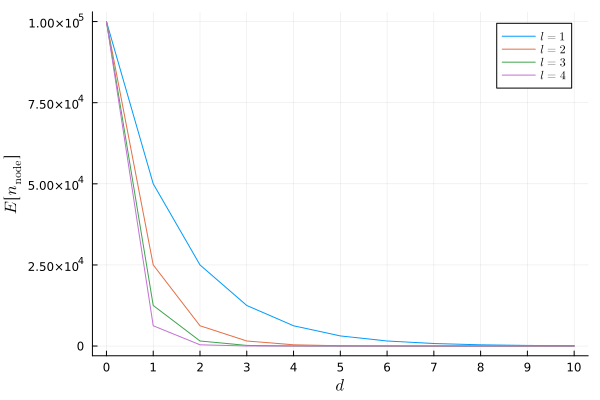
\includegraphics[width=10pc]{figures/experiments/b_vs_d.png}
  }
  \caption{ Exponential decrease of mean number of points per leaf node }
  \label{b_vs_d}
\end{figure}


\subsection{Runtime performance}
\subsubsection{Scaling with number of points}
For uniformly distributed $4$-dimensional data and $l=4$ max tree depth, the graph
\ref{scale_n} suggests that \verb|AdaptiveHierarchicalRegularBinning.jl| scales
linearly with the size $n$ of the array.

\begin{figure}[!ht]
  \centerline{
    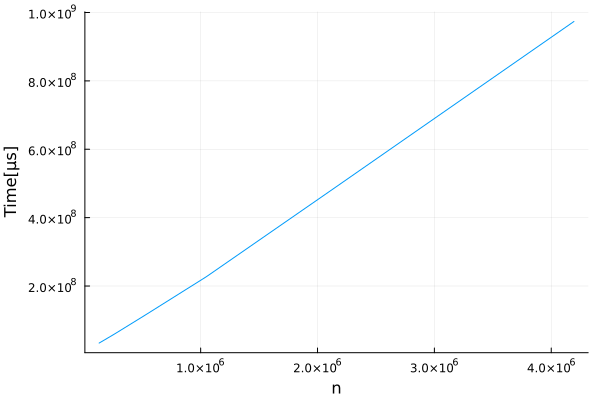
\includegraphics[width=10pc]{figures/experiments/scale_n.png}
  }
  \caption{ Linear runtime scaling }
  \label{scale_n}
\end{figure}

% TODO
% \subsubsection{Scaling with the number of dimensions}
% High dimensionality should affect the morton encoding since bit-interleaving scales
% linearly with the dimensions. The reordering should be affected slightly since each
% element


\subsubsection{Scaling with number of threads}
For uniformly distributed $n=10^6$ points of $d=10$ dimensions and a target tree of
$l=4$ levels, graph \ref{scale_t} suggests that the runtime of
\verb|AdaptiveHierarchicalRegularBinning.jl| drops exponatialy
with the number of threads.

\begin{figure}[!ht]
  \centerline{
    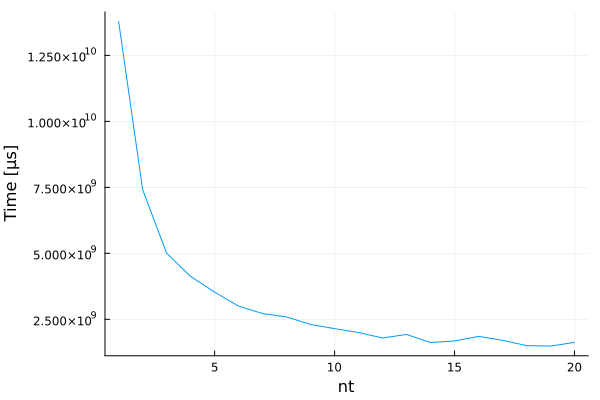
\includegraphics[width=10pc]{figures/experiments/scale_t.png}
  }
  \caption{ Parallelization scaling }
  \label{scale_t}
\end{figure}

We would expect that for a large enough number of threads the performance would worsen,
since the runtime complexity of the \verb|Countsort| algorithm suggests that if not
$n \gg t^2 \cdot r$ then the parallel variant is worse than the sequential one. Our
implementation gets around that limitation using the waterfall scheme for its
parallelization and thus for small sub-arrays the sequential variant for the
\verb|Countsort| is used.




\subsection{Uniform data 2 dimensions}

\begin{lstlisting}[language = Julia]
julia> d, n = size(X)
(2, 100000)

julia> l = 4;

julia> @time t = regural_bin(UInt128,
                             X,
                             l,
                             1;
                             dims=2);
0.025399 seconds (... 43.93% gc time)
\end{lstlisting}

For uniformly distributed data we expect that each leaf node will contain
$n_{\textrm{leaf}}$ points.
$$n_{\textrm{leaf}} = \frac{n}{2^{l\cdot d}}$$

In this case $n = 10^5$, $d = 2$ and $l = 4$. So the expected number of points within a
node is $n_{\textrm{leaf}} = \frac{10^5}{2^{4\cdot 2}} =390.625$.

\begin{figure}[!ht]
  \centerline{
    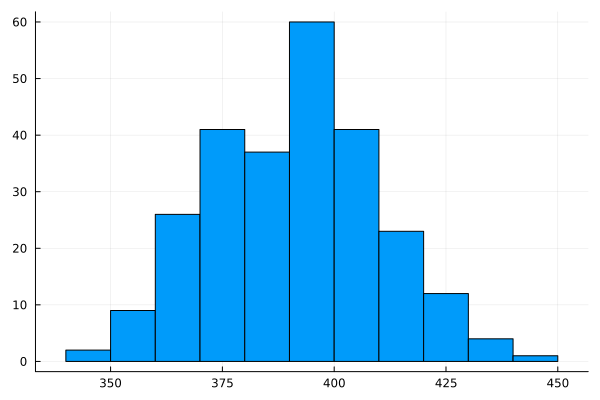
\includegraphics[width=10pc]{figures/uniform_2d/hist.png}
  }
  \caption{ Distribution of leaf node length }
  \label{uniform-2d-hist}
\end{figure}

Graph \ref{uniform-2d-hist} agrees with the theoreticaly expected value, although there
is some variance. This is to be expected, increasing the number of points will reduce
the variance then the histogram will tend more to the expected singular value.

\subsection{PBMC 30 dimensions}

The PBMC dataset exhibits outliers, which introduces challenges in the
normalization process. It causes the majority of data points to be clustered
into a single node for the first three levels of the tree. As depicted in
Figures \ref{pbmc-30-hist} (a), (b), and (c), the majority of points are
concentrated within a maximum of two nodes at these initial levels.
\\\\
However, the fourth and final level of the tree highlights the impact of the
dataset's high dimensionality. As indicated by Figure \ref{pbmc-30-hist} (d),
it becomes apparent that most points are now assigned to nodes with a length of
only $1$.

\begin{figure}[!ht]
  \centerline{
    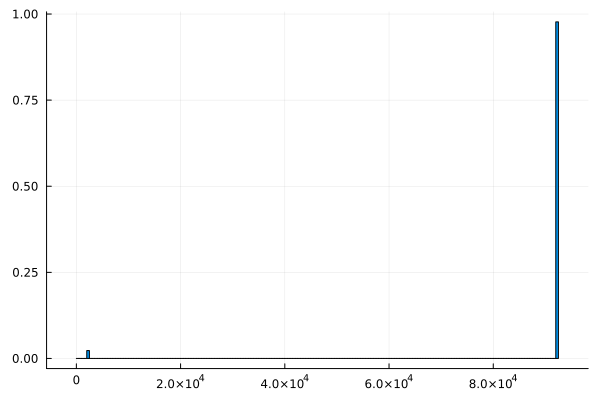
\includegraphics[width=10pc]{figures/experiments/pbmc_30/hist_1.png}
    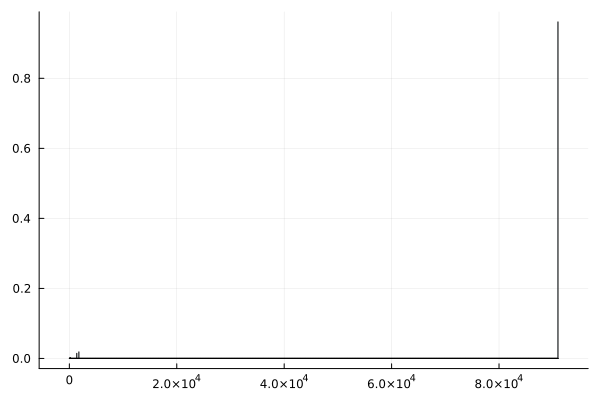
\includegraphics[width=10pc]{figures/experiments/pbmc_30/hist_2.png}
  }
  \centerline{
    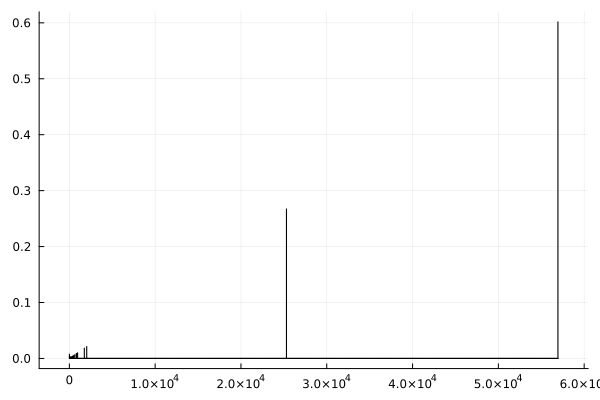
\includegraphics[width=10pc]{figures/experiments/pbmc_30/hist_3.png}
    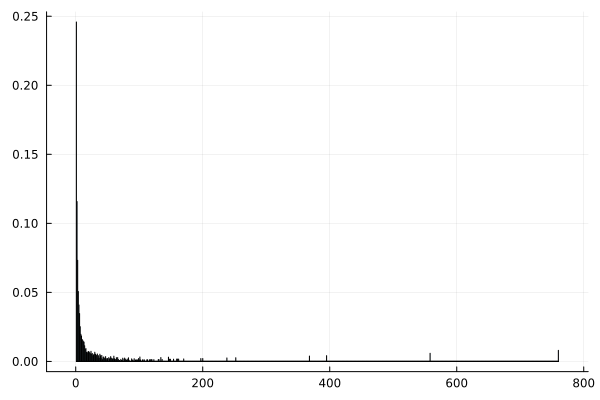
\includegraphics[width=10pc]{figures/experiments/pbmc_30/hist_4.png}
  }

  \caption{
    30-Dimensional PBMC data distribution of leaf node length for tree level
    (a) 1 (b) 2 (c) 3 (d) 4.
  }
  \label{pbmc-30-hist}
\end{figure}


\subsection{MNIST 30 dimensions}

Unlike the PBMC dataset, the MNIST dataset does not exhibit significant
outliers. As a result, the distribution between the leaf nodes in the tree
becomes more uniform. Figure \ref{mnist-30-hist} (a) reveals that a majority of
points are concentrated within leaf nodes that possess sufficiently large
lengths. This favorable grouping indicates a more balanced distribution of data
points.
\\\\
However, as we progress to higher levels of the tree, the impact of the
dataset's high dimensionality becomes apparent. Consequently, the points become
exponentially sparser, leading to the formation of singleton leaf nodes.
This observation is clearly demonstrated in Figure \ref{mnist-30-hist} (b).

\begin{figure}[!ht]
  \centerline{
    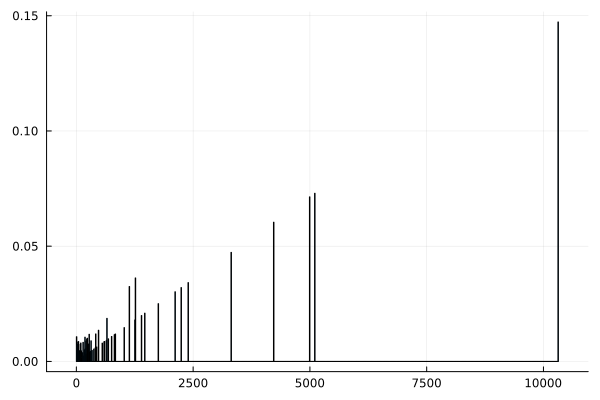
\includegraphics[width=10pc]{figures/experiments/mnist_30/hist_1.png}
    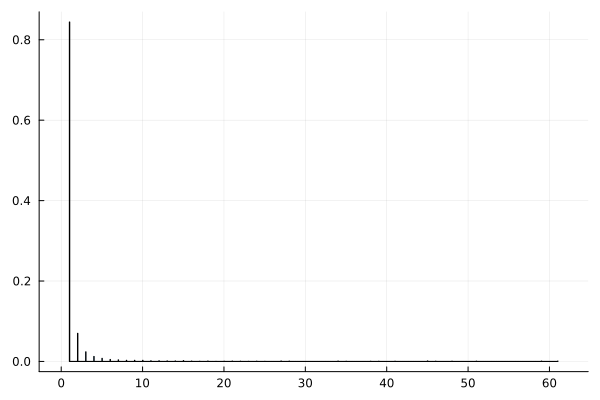
\includegraphics[width=10pc]{figures/experiments/mnist_30/hist_2.png}
  }

  \caption{
    30-Dimensional MNIST data distribution of leaf node length for tree level
    (a) 1 (b) 2
  }
  \label{mnist-30-hist}
\end{figure}

Figure \ref{mnist-30-hist-th} indicates that adjusting the \verb|Small|
threshold to approximately $10000$ causes a shift in nodes from the region of
$\geq 10000$ to the histogram's small node region, while leaving the rest of
the nodes intact. This outcome is expected because nearly all points in the
$\geq 10000$ region are mapped to a singleton node in the subsequent recursion.

\begin{figure}[!ht]
  \centerline{
    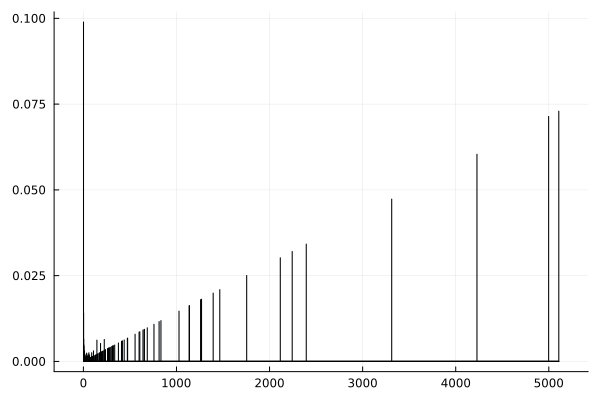
\includegraphics[width=10pc]{figures/experiments/mnist_30/hist_3.png}
  }

  \caption{
    30-Dimensional MNIST data distribution of leaf node length for tree level
    2. Using Small threshold of 10000.
  }
  \label{mnist-30-hist-th}
\end{figure}

% TODO Remove
\pagebreak
\section{Juliacon stuff, kept for reference}
\section{Introduction}

The \LaTeX{} document preparation system is a special version of the
\TeX; typesetting program where-in a collection of \TeX; commands
are added to \LaTeX{} to simplify typesetting. Importantly, it allows
the author to concentrate on the logical structure of the document
rather than its visual layout.\vskip 6pt
Moreover, \LaTeX{} provides a consistent and comprehensive document
preparation interface. There are simple-to-use commands for
generating a table of contents, lists of figures and/or tables, and indexes.
\LaTeX{} can automatically number list entries, equations, figures,
tables, and footnotes, as well as articles, sections, and subsections.
Using this numbering system, bibliographic citations, page
references, and cross references to any other numbered entity (e.g.
article, section, equation, figure, list entry, etc.) become quite simple
and straightforward. The use of \LaTeX{} document classes allows
a simple change of class to transform the appearance of your document.\vskip 6pt
\LaTeX{} is a powerful tool for managing long and complex documents.
In particular, partial processing enables long documents to
be produced article by article without losing sequential information.
The use of document classes allows a simple change of style
(or style option) to transform the appearance of your document.



\section{The JuliaCon Article Class}
\label{sec:documentclass}
%
The juliacon class file preserves the standard LATEX{} interface such
that any document that can be produced using the standard LATEX{}
article class can also be produced with the class file.\vskip 6pt
It is likely that the make up will change after file submission. For
this reason, we ask you to ignore details such as slightly long lines,
page stretching, or figures falling out of synchronization, as these
details can be dealt with at a later stage.\vskip 6pt
Use should be made of symbolic references (\verb|\ref| ) in order to
protect against late changes of order, etc.

\section{USING THE JuliaCon Article CLASS FILE}

If the file \verb|juliacon.cls|  is not already in the appropriate system directory
for \LaTeX{} files, either arrange for it to be put there or copy
it to your working directory. The \verb|juliacon|  document class is implemented
as a complete class, not a document style option. In order to
use the \verb|juliacon  document class, replace \verb|article|  by \verb|juliacon|  in the
\verb|\documentclass|  command at the beginning of your document:
\vskip 6pt
\begin{centering}
    \verb|\documentclass{article}|  \end{centering}
\vskip 6pt
replace by
\vskip 6pt
 \verb|\documentclass{juliacon}|  \vskip 6pt
In general, the following standard document \verb|style|  options should
{ \itshape not} be used with the {\footnotesize \itshape article} class file:
\begin{enumerate}
\item[(1)] \verb|10pt|,  \verb|11pt|,  \verb|12pt|   ? unavailable;
\item[(2)] \verb|twoside|  (no associated style file) ? \verb|twoside|  is the default;
\item[(3)] \verb|fleqn|, \verb|leqno|, \verb|titlepage| ? should not be used;
\end{enumerate}

\section{Additional Document Style Options}
\label{sec:additional_doc}
%
The following additional style option is available with the \verb|juliacon|  class file:
\vskip 6pt
Please place any additional command definitions at the very start of
the \LaTeX{} file, before the \verb|\begin{document}|. For example, user-defined
\verb|\def|  and \verb|\newcommand|   commands that define macros for
technical expressions should be placed here. Other author-defined
macros should be kept to a minimum.
\vskip 6pt
Commands that differ from the standard \LaTeX{} interface, or that
are provided in addition to the standard interface, are explained in
this guide. This guide is not a substitute for the \LaTeX{} manual itself.
Authors planning to submit their papers in \LaTeX{} are advised to use
\verb|juliacon.cls|  as early as possible in the creation of their files.

%
%
%
%
\begin{table*}[t]
\tabcolsep22pt
\tbl{If necessary, the tables can be extended both columns.}{
\begin{tabular}{|l|l|c|c|}\hline
Label & \multicolumn{1}{c|}{Description}
& Number of Users &
Number of Queries\\\hline
Test 1 & Training Data &
\smash{\raise-7pt\hbox{70}} & 104\\
\cline{1-2}\cline{4-4}
Test 2 & Testing Data I & & 105\\\hline
Test 3 & Testing Data II & 30 & 119\\\hline
& Total & 100 & 328\\\hline
\end{tabular}}
\label{tab:symbols}
\begin{tabnote}
This is an example of table footnote.
\end{tabnote}
\end{table*}
% \begin{figure*}[t]
% \centerline{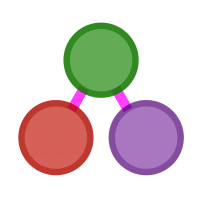
\includegraphics[width=11cm]{juliagraphs.png}}
% \caption{If necessary, the images can be extended both columns.}
%   \label{fig:sample_image}
% \end{figure*}

\section{Additional features}
\label{sec:additional_faci}
In addition to all the standard \LaTeX{} design elements, the \verb|juliacon|  class file includes the following features:
In general, once you have used the additional \verb|juliacon.cls| facilities
in your document, do not process it with a standard \LaTeX{} class
file.

\subsection{Titles, Author's Name, and Affiliation}
\label{subsub:title_auth}
The title of the article, author's name, and affiliation are used at the
beginning of the article (for the main title). These can be produced
using the following code:

\begin{verbatim}
\title{ This is an example of article title} }
\author{
   \large 1st Author \\[-3pt]
   \normalsize 1st author's affiliation  \\[-3pt]
    \normalsize 1st line of address \\[-3pt]
    \normalsize 2nd line of address \\[-3pt]
    \normalsize	1st author's email address \\[-3pt]
  \and
   \large 2nd Author \\[-3pt]
   \normalsize 2nd author's affiliation  \\[-3pt]
    \normalsize 1st line of address \\[-3pt]
    \normalsize 2nd line of address \\[-3pt]
    \normalsize	2nd author's email address \\[-3pt]
\and
   \large 3rd Author \\[-3pt]
   \normalsize 3rd author's affiliation  \\[-3pt]
    \normalsize 1st line of address \\[-3pt]
    \normalsize 2nd line of address \\[-3pt]
    \normalsize	3rd author's email address \\[-3pt]
}
\maketitle
\end{verbatim}

\subsection{Writing Julia code}

A special environment is already defined for Julia code,
built on top of \textit{listings} and \textit{jlcode}.

\begin{verbatim}
\begin{lstlisting}[language = Julia]
using Plots

x = -3.0:0.01:3.0
y = rand(length(x))
plot(x, y)
\end{lstlisting}
\end{verbatim}
\begin{lstlisting}[language = Julia]
using Plots

x = -3.0:0.01:3.0
y = rand(length(x))
plot(x, y)
\end{lstlisting}


\subsection{Abstracts, Key words, term etc...}
\label{subsub:abs_key_etc}

At the beginning of your article, the title should be generated
in the usual way using the \verb|\maketitle|  command. For genaral tem and keywords use
\verb|\terms|,
\verb|\keywords|  commands respectively. The abstract should be enclosed
within an abstract environment, All these environment
can be produced using the following code:
\begin{verbatim}
\terms{Experimentation, Human Factors}

\keywords{Face animation, image-based modelling...}

\begin{abstract}
In this paper, we propose a new method for the
systematic determination of the model's base of
time varying delay system. This method based on
the construction of the classification data related
to the considered system. The number, the orders,
the time delay and the parameters of the local
models are generated automatically without any
knowledge about the full operating range of the
process. The parametric identification of the local
models is realized by a new recursive algorithm for
on line identification of systems with unknown time
delay. The proposed algorithm allows simultaneous
estimation of time delay and parameters of
discrete-time systems. The effectiveness of
the new method has been illustrated through
simulation.
\end{abstract}

\end{verbatim}

\section{Some guidelines}
\label{sec:some_guide}
The following notes may help you achieve the best effects with the
\verb|juliacon|  class file.

\subsection{Sections}
\label{subsub:sections}
\LaTeXe{}  provides four levels of section headings and they are all
defined in the \verb|juliacon|  class file:
\begin{itemize}
\item \verb|\section|
\item \verb|\subsection|
\item \verb|\subsubsection|
\item \verb|\paragraph|
\end{itemize}
Section headings are automatically converted to allcaps style.
\subsection{Lists}
\label{sec:lists}
%
The \verb|juliacon|   class file provides unnumbered lists using the
\verb|unnumlist|  environment for example,

\begin{unnumlist}
\item First unnumbered item which has no label and is indented from the
left margin.
\item Second unnumbered item.
\item Third unnumbered item.
\end{unnumlist}
The unnumbered list which has no label and is indented from the
left margin. was produced by:
\begin{verbatim}
\begin{unnumlist}
\item First unnumbered item...
\item Second unnumbered item...
\item Third unnumbered item...
\end{unnumlist}
\end{verbatim}

The \verb|juliacon|  class file also provides hyphen list using the
\verb|itemize|  environment for example,
\begin{itemize}
\item First unnumbered bulleted item which has no label and is indented
from the left margin.
\item Second unnumbered bulleted item.
\item Third unnumbered bulleted item which has no label and is indented
from the left margin.
\end{itemize}
was produced by:
\begin{verbatim}
\begin{itemize}
\item First item...
\item Second item...
\item Third item...
\end{itemize}
\end{verbatim}

Numbered list is also provided in acmtog class file using the
enumerate environment for example,
\begin{enumerate}
\item The attenuated and diluted stellar radiation.
\item Scattered radiation, and
\item Reradiation from other grains.
\end{enumerate}

was produced by:
\begin{verbatim}
\begin{enumerate}
\item The attenuated...
\item Scattered radiation, and...
\item Reradiation from other grains...
\end{enumerate}
\end{verbatim}
\subsection{Illustrations (or figures)}
\label{subsub:sec_Illus}
The \verb|juliacon|  class file will cope with most of the positioning of
your illustrations and you should not normally use the optional positional
qualifiers on the \verb|figure|  environment that would override
these decisions.
\vskip 6pt

%
\begin{figure}[t]
\centerline{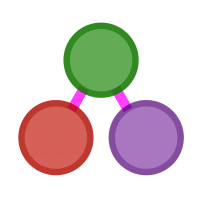
\includegraphics[width=4cm]{juliagraphs.png}}
\caption{This is example of the image in a column.}
	\label{fig:sample_figure}
\end{figure}

The figure \ref{fig:sample_figure} is taken from the JuliaGraphs
organization \footnote{https://github.com/JuliaGraphs}.

Figure captions should be \emph{below} the figure itself, therefore the
\verb|\caption|  command should appear after the figure or space left for
an illustration. For example, Figure 1 is produced using the following
commands:

\begin{verbatim}
\begin{figure}
\centerline{\includegraphics[width=20pc]{Graphics.eps}}
\caption{An example of the testing process for a
binary tree. The globa null hypothesis is tested
first at level $\alpha$ (a), and the level of
individual variables is reached last (d). Note
that individual hypotheses can be tested at
level $\alpha/4$ and not $\alpha/8$ as one might
expect at first.}
\label{sample-figure_2}
\end{figure}
\end{verbatim}
Figures can be resized using first and second argument of
\verb|\includegraphics|   command. First argument is used for modifying
figure height and the second argument is used for modifying
figure width respectively.
\vskip 6pt
Cross-referencing of figures, tables, and numbered, displayed
equations using the \verb|\label|  and \verb|\ref|   commands is encouraged.
For example, in referencing Figure 1 above, we used
\verb|Figure~\ref{sample-figure}|

 \subsection{Tables}
\label{subsub:sec_Tab}
The \verb|juliacon|   class file will cope with most of the positioning of
your tables and you should not normally use the optional positional qualifiers on the table environment which would override these
decisions. Table captions should be at the top.
\begin{verbatim}
\begin{table}
\tbl{Tuning Set and Testing Set}{
\begin{tabular}{|l|l|c|c|}\hline
Label & \multicolumn{1}{c|}{Description}
& Number of Users &
Number of Queries\\\hline
Train70 & Training Data &
\smash{\raise-7pt\hbox{70}} & 104\\
\cline{1-2}\cline{4-4}
Test70 & Testing Data I & & 105\\\hline
Test30 & Testing Data II & 30 & 119\\\hline
& Total & 100 & 328\\\hline
\end{tabular}}
\end{table}
\end{verbatim}

\begin{table}
\tbl{Tuning Set and Testing Set}{
\begin{tabular}{|l|l|c|c|}\hline
Label & \multicolumn{1}{c|}{Description}
& Number of Users &
Number of Queries\\\hline
Test 1 & Training Data &
\smash{\raise-7pt\hbox{70}} & 104\\
\cline{1-2}\cline{4-4}
Test 2 & Testing Data I & & 105\\\hline
Test 3 & Testing Data II & 30 & 119\\\hline
& Total & 100 & 328\\\hline
\end{tabular}}
\end{table}
\subsection{Landscaping Pages}
\label{subsub:landscaping_pages}
If a table is too wide to fit the standard measure, it may be turned,
with its caption, to 90 degrees. Landscape tables cannot be produced
directly using the \verb|juliacon|   class file because \TeX{} itself cannot
turn the page, and not all device drivers provide such a facility.
The following procedure can be used to produce such pages.
\vskip 6pt
Use the package \verb|rotating|   in your document and change the coding
from
\begin{verbatim}
\begin{table}...\end{table}
to
\begin{sidewaystable}...\end{sidewaystable}
and for figures
\begin{figure}...\end{figure}
to
\begin{sidewaysfigure}...\end{sidewaysfigure}
\end{verbatim}

environments in your document to turn your table on the appropriate
page of your document. For instance, the following code prints
a page with the running head, a message half way down and the
table number towards the bottom.
\begin{verbatim}
\begin{sidewaystable}
\tbl{Landscape table caption to go here.}{...}
\label{landtab}
\end{sidewaystable}
\end{verbatim}

\subsection{Double Column Figure and Tables}
\label{subsub:double_fig_tab}
For generating the output of figures and tables in double column
we can use the following coding:

\begin{enumerate}
\item For Figures:
\begin{verbatim}
\begin{figure*}...\end{figure*}
\end{verbatim}
\item For landscape figures:
\begin{verbatim}
\begin{sidewaysfigure*}...\end{sidewaysfigure*}
\end{verbatim}
\item For Tables:
\begin{verbatim}
\begin{table*}...\end{table*}
\end{verbatim}
\item For landscape tables:
\begin{verbatim}
\begin{sidewaystable*}...\end{sidewaystable*}
\end{verbatim}
\end{enumerate}

\subsection{Typesetting Mathematics}
\label{subsub:type_math}
The \verb|juliacon| class file will set displayed mathematics with center to
the column width, provided that you use the \LaTeXe{} standard of
open and closed square brackets as delimiters.
The equation
\[
\sum_{i=1}^p \lambda_i = (S)
\]

was typeset using the acmtog class file with the commands

\begin{verbatim}
\[
\sum_{i=1}^p \lambda_i = (S)
\]
\end{verbatim}

For display equations, cross-referencing is encouraged. For example,
\begin{verbatim}
\begin{equation}
(n-1)^{-1} \sum^n_{i=1} (X_i - \overline{X})^2.
\label{eq:samplevar}
\end{equation}
Equation~(\ref{eq:samplevar}) gives the formula for
sample variance.
\end{verbatim}
The following output is generated with the above coding:
\begin{equation}
(n-1)^{-1} \sum^n_{i=1} (X_i - \overline{X})^2.
\label{eq:samplevar}
\end{equation}
Equation~(\ref{eq:samplevar}) gives the formula for
sample variance.


\subsection{Enunciations}
\label{subsub:enunciation}
The \verb|juliacon|   class file generates the enunciations with the help of
the following commands:
\begin{verbatim}
\begin{theorem}...\end{theorem}
\begin{strategy}...\end{strategy}
\begin{property}...\end{property}
\begin{proposition}...\end{proposition}
\begin{lemma}...\end{lemma}
\begin{example}...\end{example}
\begin{proof}...\end{proof}
\begin{definition}...\end{definition}
\begin{algorithm}...\end{algorithm}
\begin{remark}...\end{remark}
\end{verbatim}
The above-mentioned coding can also include optional arguments
such as
\begin{verbatim}
\begin{theorem}[...]. Example for theorem:
\begin{theorem}[Generalized Poincare Conjecture]
Four score and seven ... created equal.
\end{theorem}
\end{verbatim}

\begin{theorem}[Generalized Poincare Conjecture]
Four score and seven years ago our fathers brought forth,
upon this continent, a new nation, conceived in Liberty,
 and dedicated to the proposition that all men are
created equal.
\end{theorem}


\subsection{Extract}
\label{subsub:extract}
Extract environment should be coded within
\begin{verbatim}
\begin{extract}..\end{extract}
\end{verbatim}

\subsection{Balancing column at last page}
\label{subsub:Balance}
For balancing the both column length at last page use :
\begin{verbatim}
\vadjust{\vfill\pagebreak}
\end{verbatim}

%\vadjust{\vfill\pagebreak}

at appropriate place in your \TeX{} file or in bibliography file.

\section{Handling references}
\label{subsub:references}
References are most easily (and correctly) generated using the
BIBTEX, which is easily invoked via
\begin{verbatim}
\bibliographystyle{juliacon}
\bibliography{ref}
\end{verbatim}
When submitting the document source (.tex) file to external
parties, the ref.bib file should be sent with it.
\cite{bezanson2017julia}

% **************GENERATED FILE, DO NOT EDIT**************

\bibliographystyle{juliacon}
\bibliography{ref.bib}


\end{document}

% Inspired by the International Journal of Computer Applications template
